\section{Motivation for Training DNN on CPU}
%%%\textcolor{jie}{As the DNN model becoming lager and deeper, memory capacity in training platform becomes critical in DNN training procedure. Given the size of DNN model and the size of training batches, the minimal memory usage in training platform can be calculated. A typical modern GPU has 12 GB to 16GB DRAM. Limited memory size in GPU can be harmful to large DNN model training accuracy because the maximum batch size that can fit in memory is too small.}

\textcolor{check}{Since modern HM typically serves CPU, we focus on CPU. Using CPU for training is commonly supported by hardware vendors (e.g., Intel MKL-DNN~\cite{intelMKL} and ARM Compute Library~\cite{arm_cl}), and has the following four benefits. (1) The trend of democratizing DNN~\cite{democratization_ai} makes CPU an appealing solution. Compared with GPU, CPU is more approachable and affordable, especially for personal users or small-sized enterprises; (2) Some data centers do not have GPU and simply use CPU for training~\cite{lbnl_cori, tacc_stampede, 8658402, Kurth:2018:EDL:3291656.3291724, Mathuriya:2018:CUD:3291656.3291743,  tacc_ml_CPU_training}; (3) For those DNN models that lack thread level parallelism, GPU can perform worse than CPU (e.g., \cite{DBLP:journals/corr/ChengKHSCAACCIA16, Hasselt:2016:DRL:3016100.3016191,mlsys19:chen});  
%(e.g., the wide-and-deep model~\cite{DBLP:journals/corr/ChengKHSCAACCIA16} and DQN~\cite{Hasselt:2016:DRL:3016100.3016191}); 
(4) On a public cloud, CPU is cheaper than GPU. For example, on the google cloud, one vCPU is only 1/46 and 1/78 of NIVIDA P100 and V100 GPU, in terms of cost per hour.} %When the training times on CPU and GPU are comparable, using CPU can be easily more cost effective.}



\textcolor{check}{Besides the above reasons, we find big benefits of training DNN on CPU with large memory capacity, compared with on GPU with smaller memory capacity. We use training BERT~\cite{devlin2018bert} as an example to show the benefits. We follow the common practice to train a pre-trained BERT on CPU or GPU. In the common practice, a general purpose BERT model is trained from scratch using large-scale computing resources; Then the user trains the pre-trained BERT model with a user-specific dataset. We focus on the user training process, because it happens much more frequently than pre-training.}

%\textcolor{jie}{We study the fine-tuning procedure for BERT~\cite{devlin2018bert}, the state-of-the-art Natural Language Processing (NLP) model. BERT model training, including pre-training and fine-tuning. Pre-training aims to train a general-purpose model on a large text corpus, which usually takes several days in with tens of TPU chips but only happens once for each language. While fine-tuning fine-tunes the pre-trained model for a particular task or for the future extension with a specific dataset. The fine-tuning is inexpensive in computation comparing with pre-training. However, due to the size of the BERT model does not reduce in fine-tuning, the memory consumption of fine-tuning is still large. Fine-tuning happens more  frequent than pre-training, and often happen in GPU and CPU since they are easy to access compared with TPUs.}


\textcolor{check}{
We train the BERT-Large model~\cite{devlin2018bert}.  Table~\ref{tab:hw_gpu} shows the hardware details. 
Because of small memory capacity on GPU, the maximum batch size for training is 5, but \textcolor{red}{we use 4 because it leads to the shortest training convergence time on GPU}. On CPU, we use 16 and 32 as the batch size, following the common practice~\cite{devlin2018bert}. We evaluate three common learning rates 5e-5, 3e-5, and 2e-5 suggested in~\cite{devlin2018bert}, but present the results that use one of the three rates that leads to the fastest training convergence.}

%\textcolor{jie}{We compare the BERT-Large model~\cite{devlin2018bert} fine-tuning procedure in CPU and GPU. Table~\ref{tab:hw_gpu} shows the hardware details. Due to the limited memory size in GPU, we chose 4 as the batch size for BERT-Large model fine-tuning on GPU, and the maximum batch size fit in experimental GPU is 5. The DRAM size on CPU much larger, and we choose 16 and 32 as the batch size for BERT-Large model fine-tuning on CPU. We choose three different learning rates 5e-5, 3e-5, 2e-5 as suggested in BERT~\cite{devlin2018bert} and present the best configuration for each batch size(i.e., the learning rate to converge fastest) for the following comparison.}
%%%Due to the limited memory size in GPU, the maximum batch size is small for fine-tuning on a GPU is about 4 to 6.

\begin{table}[t]
\centering
%\scriptsize
%\small
%\vspace{-3pt}
\caption{\textcolor{check}{CPU and GPU platforms for training.}}
\vspace{-5pt}
\begin{tabular}{ll}
\hline
CPU: Intel Xeon E5-2670 CPU & RAM : 64GB\\ %\phantom{LA}  @2.30GHz
GPU: Nvidia TITAN XP GPU & RAM : 11427MB\\
\hline
\end{tabular}
\vspace{-5pt}
%\vspace{-25pt}
\label{tab:hw_gpu}
\end{table}

\begin{figure}[!t]
\centering
%\vspace{-20pt}
%\includegraphics[width=0.48\textwidth]{figures/mem_size.pdf}
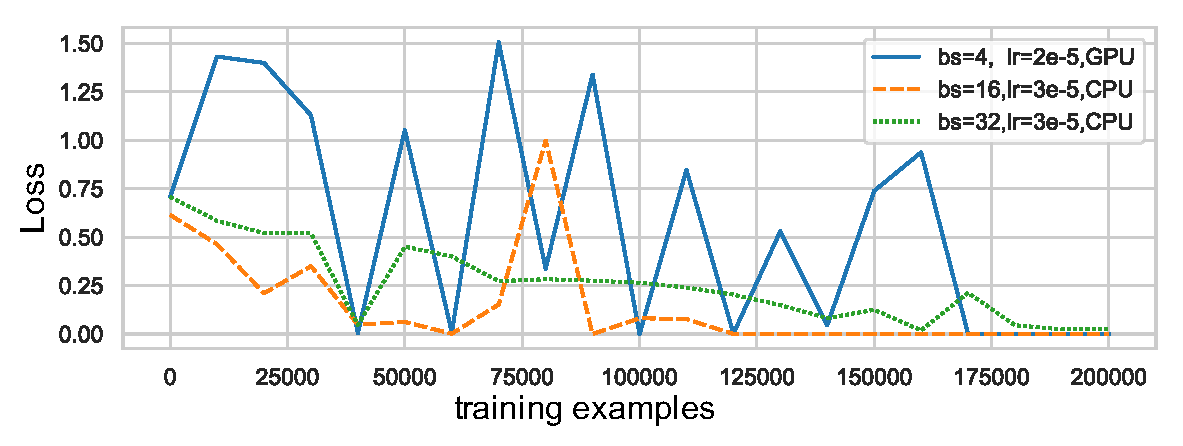
\includegraphics[width=0.48\textwidth]{figures/bert_curve.pdf}
%\vspace{-25pt}
%\caption{\name tensor access histogram.  x-axis shows tensor access frequency and y-axis shows the number of tensors.}
%\caption{\textcolor{jie}{BERT training loss curve with different batch size. ``bs'' and ``lr'' stand for `batch size' and  ``learning rate'' respectively.}}
\vspace{-20pt}
\caption{\textcolor{check}{BERT training loss curves. ``bs'' and ``lr'' stand for `batch size' and  ``learning rate'' respectively.}}
\vspace{-5pt}
\label{fig:bert_motivation}
\end{figure}

\begin{table}[t]
\small
\caption{\textcolor{check}{Convergence times on five datasets in GLUE.}}
\vspace{-5pt}
\begin{tabular}{|c|c|c|c|c|c|}
\hline
\textbf{Batch size}      & \textbf{MRPC} & \textbf{RTE} & \textbf{STS-B} & \textbf{CoLA} & \textbf{SST-2} \\ \hline
\textbf{4  (GPU)}  & 39min         & 48min        & 163min         & 209min        & 187min         \\ \hline
\textbf{16 (CPU)} & 110min        & 85min        & 267min         & 219min        & 540min         \\ \hline
\textbf{32 (CPU)} & 106min        & 104min       & 282min         & 237min        & 539min         \\ \hline
\end{tabular}
\vspace{-5pt}
\label{tab:glue_bench}
\end{table}


\textcolor{check}{
Figure~\ref{fig:bert_motivation} shows the training curve when we use the CoLA dataset in GLUE benchmark~\cite{wang-etal-2018-glue}. We have two observations.}

\begin{itemize} %[leftmargin=*]
    \item \textcolor{check}{Training on GPU converges much slower than that on CPU, and consumes 1.75x more training examples;}
    %%%\textcolor{jie}{Training on GPU consumes much more training examples(1.75x on CoLA dataset) to get converge than training on CPU.}
    \item \textcolor{check}{Convergence times on GPU (209 mins) and CPU (219 mins) are comparable (see Table~\ref{tab:glue_bench})}. 
\end{itemize}

\textcolor{check}{
We test five datasets in GLUE and have the same observations. Table~\ref{tab:glue_bench} summarizes the training convergence times. The above observations are due to the fact that GPU has a much smaller memory capacity and has to use a smaller batch size for training. Larger memory capacity on CPU brings obvious benefits to train large machine learning models, which drives our study on runtime data management on HM on CPU.
}




\begin{comment}
\textcolor{jie}{Figure~\ref{fig:bert_motivation} shows the training curve of the BERT-Large fine-tuning procedure with the CoLA task in GLUE benchmark~\cite{wang-etal-2018-glue}. When fine-tuning happens on GPU, the model converges slowly, and the fine-tuning procedure is unstable since the batch size is too small. Using CPU for BERT-Large model fine-tuning can enable larger batch sizes. Fine-tuning on GPU needs 1.75x training examples to get converged comparing with fine-tuning the model on CPU with batch size as 16.
%%%Comparing with training on GPU, training on CPU with batch size as 16 uses half of training examples to get the stable point.
%%%converges faster than fine-tuning the model on GPU.
We further compare the converge time training on different platforms. Fine-tuning BERT-Large model with CoLA on CPU uses 3.7 hours to converge, while uses 3.5 hours on GPU with much better hardware parallelism. 
%%%The result for other tasks in the GLUE benchmark does not show because of space limitation. 
We test five datasets in GLUE benchmark and the result shows in table~\ref{tab:glue_bench}. 
We found that using CPU for fine-tuning can enable large batch sizes and make training procedures more stable comparing with training on GPU. With the best configuration(both CPU and GPU), CPU training time is
about 1.06x to 3x compared with GPU training time to converge.
}

\textcolor{jie}{Our experiments show that training DNN on CPU can be benefit for CPU large memory capacity and enable larger batch sizes, which is helpful for fast convergence and stable training. 
Besides, for some DNN whose training procedure does not involve intensive computation, the training time on CPU is comparable with training time on GPU, with much less cost.
It is important to explore memory management on CPU to maximize the benefit of the DNN training on CPU.
}

\end{comment}